
 \section{Generate A Table Of Contents}
\begin{itemize}
	\item Menurut Wikipedia \par

LaTeX adalah bahasa markup atau sistem penyiapan dokumen untuk peranti lunak TeX. Tex merupakan program komputer yang digunakan untuk membuat typesetting suatu dokumen, atau membuat formula matematika. LaTeX memungkinkan penulis/penggunanya untuk melakukan typesetting dan mencetak hasil kerjanya dalam bentuk tipografi yag terbaik. Oleh karenanya LaTeX paling banyak digunakan oleh para matematikawan, ilmuwan, insinyur, akademisi, dan profesional lainnya.\par

\vspace{\baselineskip}
	\item Secara Umum\par

LaTeX adalah word processor (pengolah kata, pembuat dokumen) mirip Microsoft Word. LaTeX lebih cocok digunakan untuk membuat dokumen yang panjang, bukan yang pendek. Dengan begitu, keampuhan LaTeX dapat ditampilkan. LaTeX juga lebih dapat menampilkan kecanggihannya ketika kita menulis scientific document.\par
\vspace{\baselineskip}

LATEX adalah alat yang hebat untuk membuat dokumen, ini berdasarkan gagasan wysiwym (what you see is what you mean), idea -> apa yang anda lihat adalah apa yang anda maksud), artinya kita hanya fokus pada isi dokumen saja dan computer yang akan mengurus formatnya. Dengan LATEX sangat mudah untuk membuat bahan yang tampak profesional.\par

\vspace{\baselineskip}

Contoh kode program Generate Table Of Content.\par

\begin{verbatim}
\documentclass{article}
\begin{document}
\tableofcontents
\newpage
\section{Section}
Dummy text
\subsection{Subsection}
Dummy text
\end{document}
\end{verbatim}

Hasil dari kode program di atas seperti di bawah ini: \par

\begin{itemize}
	\item Hasil kode program
\end{itemize}
\begin{figure}[ht]
	\centerline{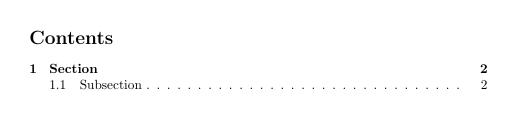
\includegraphics[width=0.70\textwidth]{gambar/Conten}}
	\caption{Hasil Kode Program}
	\label{Hasil Kode Program}
\end{figure}

\vspace{\baselineskip}

\begin{itemize}
	\item Latex
\end{itemize}
\begin{figure}[ht]
	\centerline{\includegraphics[width=0.40\textwidth]{gambar/Latex}}
	\caption{Latex}
	\label{Latex}
\end{figure}

 \par
\vspace{\baselineskip}
Artikel ini menyajikan dasar-dasar untuk membuat dokumen.\par

\hspace*{0.5in}Isi\par

\hspace*{0.5in}1. Perkenalan\par

\hspace*{0.5in}2. Pembukaan dokumen\par

\hspace*{0.5in}3. Menampilkan judul dokumen Anda\par

\hspace*{0.5in}4. Format dasar: abstrak, paragraf dan baris baru\par

\hspace*{0.5in}5. Komentar\par

\hspace*{0.5in}6. Panduan Referensi\par

\vspace{10pt}

	\item {\fontsize{14pt}{14pt}\selectfont \textbf{Pengantar/Perkenalan}}\par
\vspace{\baselineskip}
Mari kita mulai dengan contoh kerja yang paling sederhana:\par

\hspace*{0.5in}$\setminus$ documenkelas $ \{ $arttikel$ \} $\par

\hspace*{0.5in}$\setminus$ begin $ \{ $documen$ \} $\par
\vspace{\baselineskip}

\hspace*{0.5in}Dokumen pertama ini adalah contoh sederhana, dengan no parameter tambahan atau paket \hspace*{0.5in}disertakan.\par

\hspace*{0.5in}$\setminus$ end $ \{ $document$ \} $\par

Baris pertama kode menyatakan jenis dokumen, dalam hal ini adalah sebuah artikel. Kemudian disertakan dalam tag $\setminus$ begin $ \{ $dokumen$ \} $ $\setminus$ end $ \{ $document$ \} $ dan kita harus menulis teks dokumen.\par

\vspace{10pt}
	\item {\fontsize{14pt}{14pt}\selectfont \textbf{Pembukaan Dokumen}}\par
\vspace{\baselineskip}
Pada contoh sebelumnya, teks dimasukkan setelah perintah $\setminus$ begin $ \{ $document$ \} $. Bagian dari file .tex anda sebelum titik ini disebut pendahuluan. Dalam basa-basi anda menentukan jenis dokumen yang anda tulis, bahasa dan beberapa elemen lainnya. Misalnya, pendahuluan dokumen normal akan terlihat seperti ini:\par
\vspace{\baselineskip}
\hspace*{0.5in}$\setminus$ documentclass [12pt, letterpaper] $ \{ $article$ \} $\par
\vspace{\baselineskip}
\hspace*{0.5in}$\setminus$ usepackage [utf8] $ \{ $inputenc$ \} $\par

\hspace*{0.5in}$\setminus$ title $ \{ $Dokumen pertama$ \} $\par
\vspace{\baselineskip}

$\setminus$ author $ \{ $Hubert Farnsworth $\setminus$ thanks $ \{ $didanai oleh tim ShareLaTeX$ \} $$ \} $\par

\hspace*{0.5in}$\setminus$ tanggal $ \{ $September 2017$ \} $\par
\vspace{\baselineskip}
Berikut penjelasan rinci setiap baris:\par
\vspace{\baselineskip}
$\setminus$ documentclass [12pt, letterpaper] $ \{ $article$ \} $\par
\vspace{\baselineskip}
\hspace*{0.5in}Seperti dikatakan sebelumnya, ini mendefinisikan jenis dokumen. Beberapa parameter tambahan di dalam kurung dan dipisahkan koma dapat dilewatkan ke perintah. Pada contoh, parameter tambahan mengatur ukuran font (12pt) dan ukuran kertas (letterpaper). Tentu saja ukuran font lainnya (9pt, 11pt, 12pt) bisa digunakan, ukuran defaultnya adalah 10pt. Sedangkan untuk ukuran kertas, nilai lain yang mungkin adalah a4paper dan legalpaper; \par
\vspace{\baselineskip}
$\setminus$ usepackage [utf8] $ \{ $inputenc$ \} $\par

\hspace*{0.5in}Ini adalah pengkodean untuk dokumen. Dapat dihilangkan atau diubah ke pengkodean lain tapi utf-8 direkomendasikan. Kecuali anda secara khusus memerlukan pengkodean lain, atau jika anda tidak yakin akan hal itu, tambahkan baris ini ke pendahuluan.\par
\vspace{\baselineskip}
Tiga baris berikutnya bersifat deskriptif. Bagaimanapun, Anda bisa melihat deskripsi tentang apa yang sebenarnya mereka lakukan di bagian selanjutnya.\par
\vspace{\baselineskip}
Parameter penting lainnya yang bisa dilewatkan ke perintah documentclass adalah twocolumn jika anda menginginkan teks anda dalam format dua kolom dan dua huruf untuk pencetakan lembar kertas dua sisi.\par
\vspace{\baselineskip}
\vspace{10pt}
	\item {\fontsize{14pt}{14pt}\selectfont \textbf{Menampilkan Judul Dokumen}}\par
\vspace{\baselineskip}
Untuk menampilkan judul dokumen anda, anda harus mendeklarasikan komponennya dalam pembukaan dan kemudian menggunakan beberapa kode tambahan:\par
\vspace{\baselineskip}
\hspace*{0.5in}$\setminus$ documentclass [12pt, letterpaper, twoside] $ \{ $article$ \} $\par

\hspace*{0.5in}$\setminus$ usepackage [utf8] $ \{ $inputenc$ \} $\par

\hspace*{0.5in}$\setminus$ title $ \{ $Dokumen pertama$ \} $\par
\vspace{\baselineskip}
$\setminus$ author $ \{ $Hubert Farnsworth $\setminus$ thanks $ \{ $didanai oleh tim ShareLaTeX$ \} $$ \} $\par
\vspace{\baselineskip}
\hspace*{0.5in}$\setminus$ tanggal $ \{ $September 2017$ \} $\par

\hspace*{0.5in}$\setminus$ begin $ \{ $document$ \} $\par

\hspace*{0.5in}$\setminus$ begin $ \{ $titlepage$ \} $\par

\hspace*{0.5in}$\setminus$ maketitle\par

\hspace*{0.5in}$\setminus$ end $ \{ $titlepage$ \} $\par
\vspace{\baselineskip}
Dalam dokumen ini ada beberapa paket dan parameter tambahan ditambahkan. Ada paket encoding sebuah parameter pageize dan fontsize.\par

\hspace*{0.5in}$\setminus$ end $ \{ $document$ \} $\par

Ada satu blok dengan tiga baris dalam basa-basi yang menentukan informasi apa yang akan dimasukkan ke dalam halaman judul.\par

\hspace*{0.5in}$\setminus$ title $ \{ $Dokumen pertama$ \} $\par

\hspace*{0.5in}Inilah judulnya.\par

\hspace*{0.5in}$\setminus$ author $ \{ $Hubert Farnsworth$ \} $\par

Di sini anda memasukkan nama Pengarang, dan sebagai parameter opsional, anda dapat menambahkan perintah berikutnya:\par
\vspace{\baselineskip}
\hspace*{0.5in}$\setminus$thanks\par

\hspace*{0.5in}$\setminus$ tanggal $ \{ $September 2017$ \} $\par

Anda dapat memasukkan tanggal secara manual atau menggunakan perintah $\setminus$ hari ini sehingga tanggal akan diperbarui secara otomatis pada saat anda mengkompilasi dokumen. \par
\vspace{\baselineskip}
\hspace*{0.5in}$\setminus$ begin $ \{ $titlepage$ \} $ $\setminus$ end $ \{ $titlepage$ \} $\par

Ini menyatakan lingkungan, blok kode dengan perilaku tertentu tergantung pada jenisnya. Dalam hal ini apapun yang anda sertakan di lingkungan judul halaman ini akan muncul di halaman pertama dokumen anda.\par
\vspace{\baselineskip}
\hspace*{0.5in}$\setminus$ maketitle\par

Perintah ini akan mencetak judul, penulis dan tanggal dalam format yang ditunjukkan. Jika tidak tertutup dalam lingkungan judul halaman, dokumen itu akan ditampilkan di awal dokumen, di atas baris pertama.\hspace*{0.5in}\par
\vspace{\baselineskip}
\vspace{10pt}
	\item {\fontsize{14pt}{14pt}\selectfont \textbf{Format Dasar: Abstrak, Paragraf dan Baris Baru}}\par
\vspace{\baselineskip}
Semua yang termasuk dalam perintah $\setminus$ begin $ \{ $document$ \} $ $\setminus$ end $ \{ $document$ \} $ akan diberikan dalam dokumen akhir.\par
\vspace{\baselineskip}
\hspace*{0.5in}$\setminus$ begin $ \{ $document$ \} $\par

\hspace*{0.5in}$\setminus$ begin $ \{ $abstract$ \} $\par
\vspace{\baselineskip}
\hspace*{0.5in}Ini adalah paragraf sederhana di awal dokumen. Pengantar singkat tentang subjek utama.\par
\vspace{\baselineskip}
\hspace*{0.5in}$\setminus$ end $ \{ $abstrak$ \} $\par

Dalam dokumen ini ada beberapa paket dan parameter tambahan ditambahkan. Ada paket encoding sebuah parameter pageize dan fontsize. Baris ini akan memulai Paragraf kedua. Dan saya bisa rem $\setminus$ $\setminus$ the garis $\setminus$$\setminus$ dan lanjutkan di baris baru.\par
\vspace{\baselineskip}
\hspace*{0.5in}$\setminus$ end $ \{ $document$ \} $\par

Dalam dokumen ilmiah, ini adalah praktik umum untuk menyertakan ikhtisar singkat pokok utama makalah ini. Di LATEX ada lingkungan abstrak untuk ini. Lingkungan abstrak akan memasukkan teks dalam format khusus di bagian atas dokumen anda.\par
\vspace{\baselineskip}
Saat menulis isi dokumen anda, jika anda perlu memulai paragraf baru anda harus menekan tombol "Enter" dua kali (untuk memasukkan baris kosong ganda). Perhatikan bahwa paragraf memiliki spasi putih sebelum baris pertama.\par
\vspace{\baselineskip}
Untuk memulai baris baru tanpa benar-benar memulai paragraf baru masukkan titik putus, ini bisa dilakukan oleh $\setminus$$\setminus$ (garis miring terbalik ganda) atau perintah $\setminus$ new line.\par
\vspace{\baselineskip}
\vspace{10pt}
	\item {\fontsize{14pt}{14pt}\selectfont \textbf{Komentar}}\par
\vspace{\baselineskip}
Terkadang perlu menambahkan komentar ke kode LATEX agar mudah dibaca. Ini sangat mudah, beri$\%$ sebelum komentar dan LATEX akan mengabaikan teks itu.\par
\begin{verbatim}

\documentclass \{article} 

\usepackage [utf8] {inputenc} % kodifikasi dokumen

\usepackage {comment} 

Di sini mulai isi dokumen

\begin {document}

\end{verbatim}

\hspace*{0.5in}Dokumen ini berisi banyak komentar, bukan dari mereka akan tetapi muncul disini, hanya teks ini saja. Dokumen ini berisi banyak komentar, bukan dari mereka akan tetapi muncul disini, hanya teks ini saja.\par

\hspace*{0.5in}$\setminus$ begin $ \{ $comment$ \} $\par

\hspace*{0.5in}Teks ini tidak akan muncul dalam pdf yang dikompilasi ini hanya komentar multi-line Misalnya, komentari slow-rendering sambil mengerjakan draft.\par

\hspace*{0.5in}$\setminus$ end $ \{ $comment$ \} $\par

\hspace*{0.5in}$\setminus$ end $ \{ $document$ \} $\par
\vspace{\baselineskip}
Pada bagian terakhir dari contoh, Anda dapat melihat lingkungan komentar, ini membantu dalam komentar multi-baris dan bukan menempatkan$\%$ di awal setiap baris. Agar ini bisa berhasil, Anda harus menambahkan baris berikutnya:\par
\vspace{\baselineskip}
\hspace*{0.64in}$\setminus$usepackage$ \{ $comment$ \} $\par

Simbol$\%$ adalah karakter reserved, jika Anda benar-benar membutuhkan simbol ini untuk dicetak dalam dokumen Anda, gunakan $\setminus$$\%$.\par
\vspace{\baselineskip}
\vspace{10pt}
	\item {\fontsize{14pt}{14pt}\selectfont \textbf{Panduan Referensi}}\par
\vspace{\baselineskip}
Jenis dokumen tersedia dalam perintah $\setminus$ documentclass.\par
\vspace{\baselineskip}
Tipe dokumen\hspace*{0.5in}Deskripsi\hspace*{0.5in}\par

-Artikel\hspace*{0.5in}-Dokumen pendek dan artikel yang paling umum digunakan.\par

-Laporan\hspace*{0.5in}-Untuk dokumen dan disertasi yang lebih panjang.\par

-Buku\hspace*{0.6in}-Untuk menulis buku\par

-Surat\hspace*{0.6in}-Untuk surat berbagai macam\hspace*{0.5in}\par

-Slide\hspace*{0.6in}-Untuk slide, namun jarang digunakan\par

-Beamer\hspace*{0.5in}-Lihat dokumentasi beamer untuk deskripsi yang lebih baik\par
\vspace{\baselineskip}
Karakter yang dilindungi\par
\vspace{\baselineskip}
Karakter simbol berikut dicadangkan oleh LATEX karena mereka mengenalkan perintah dan memiliki arti khusus.\par

$\#$ $\$$$\%$ $ \string^ $ $\&$ $ \_ $ $ \{ $$ \} $ $ \sim $ $\setminus$\par

\vspace{10pt}
	\subsection{Paragraf Baru}

Untuk memulai paragraf baru di LATEX, seperti yang dikatakan sebelumnya, Anda harus membiarkan baris kosong di antaranya. Ada cara lain untuk memulai paragraf baru, lihat cuplikan kode berikut.\par
\vspace{\baselineskip}
Ini teks di paragraf pertama. Ini teksnya terlebih dahulu. Ini adalah teks di paragraf pertama. $\setminus$par\par
\vspace{\baselineskip}
Ini adalah teks dalam paragraf kedua. Ini adalah teks kedua. Ini adalah teks dalam paragraf kedua.\par

Seperti yang bisa anda lihat, perintah $\setminus$ par juga untuk memulai paragraf baru.\par

\vspace{10pt}
	\subsection{Paragraf Alignment (Pembenaran Teks)}

Paragraf di LaTeX sepenuhnya dibenarkan, yaitu dengan margin kiri dan kanan. Jika anda ingin mengubah sebuah paragraf, LATEX memiliki tiga lingkungan : center, flushleft dan flushright.\par
\vspace{\baselineskip}
\hspace*{0.5in}$\setminus$ begin $ \{ $flushleft$ \} $\par

`` LaTeX adalah sistem persiapan dokumen dan markup dokumen bahasa. \par
\vspace{\baselineskip}
LaTeX menggunakan program typesetting TeX untuk pemformatan outputnya, dan ditulis sendiri dalam bahasa makro TeX.\par
\vspace{\baselineskip}
LaTeX bukan nama program pengeditan tertentu, namun merujuk ke konvensi pengkodean atau penandaan yang digunakan dalam dokumen LaTeX ".\par

\hspace*{0.5in}$\setminus$ end $ \{ $flushleft$ \} $\par
\vspace{\baselineskip}
Flushleft kiri-membenarkan paragraf. Untuk right-justify gunakan flushright sebagai gantinya.\par
\vspace{\baselineskip}
Tulisan yang disebutkan di atas didasarkan pada perintah saklar: $\setminus$ raggedright (setara dengan flushleft), $\setminus$ raggedleft (setara dengan flushright) dan keterpusatan (setara dengan pusat). \par
\vspace{\baselineskip}
Perintah switch mengalihkan penyelarasan dari titik di mana ia dimasukkan ke bagian akhir dokumen, kecuali jika ada perintah saklar lain yang dimasukkan.\par

\vspace{10pt}
	\subsection{Paragraf Indentasi}

Secara default, LATEX tidak menyertakan paragraf pertama dari sebuah bagian. Ukuran indentasi paragraf berikutnya ditentukan oleh parameter. \par

\hspace*{0.5in}$\setminus$ setlength $ \{ $$\setminus$ parindent$ \} $ $ \{ $10ex$ \} $\par
\vspace{\baselineskip}
\vspace{\baselineskip}
Ini teks di paragraf pertama. Ini teksnya terlebih dahulu. Ini teks di paragraf pertama. $\setminus$par\par
\vspace{\baselineskip}
\hspace*{0.5in}$\setminus$ noindent$\%$ Paragraf berikutnya tidak menjorok\par
\vspace{\baselineskip}
Ini teks di paragraf kedua. Ini teks kedua. Ini teks dalam paragraf kedua.\par
\vspace{\baselineskip}
Panjang default parameter ini ditentukan oleh kelas dokumen yang digunakan. Hal ini memungkinkan untuk mengubah ukuran indent paragraf dengan menggunakan perintah $\setminus$ setlength. Pada paragraf $\setminus$ setlength $ \{ $$\setminus$ parindent$ \} $ $ \{ $10ex$ \} $ akan menjorok 10ex (sebuah "ex" sama dengan panjang "x" pada font saat ini)\par
\vspace{\baselineskip}
Jika anda ingin membuat paragraf non-indentasi, anda dapat menggunakan perintah $\setminus$ noindent pada awal paragraf.\par
\vspace{\baselineskip}
Jika anda ingin indentasi paragraf yang tidak indentasi, anda bisa menggunakan $\setminus$ indent di atasnya. Perlu dicatat bahwa perintah ini hanya akan berpengaruh bila $\setminus$ parindent tidak diset ke nol.\par
\vspace{\baselineskip}
\vspace{10pt}
	\item {\fontsize{14pt}{14pt}\selectfont \textbf{Jeda Baris}}\par
\vspace{\baselineskip}
Ada lebih dari satu cara untuk memasukkan jeda baris.\par
\vspace{\baselineskip}
\hspace*{0.5in}$\setminus$ documentclass $ \{ $article$ \} $\par

\hspace*{0.5in}$\setminus$ usepackage [utf8] $ \{ $inputenc$ \} $\par

\hspace*{0.5in}$\setminus$ begin $ \{ $document$ \} $\par
\vspace{\baselineskip}
Sesuatu dalam dokumen ini tidak berisi informasi dan tujuannya adalah untuk memberi contoh bagaimana cara menyisipkan spasi dan garis putus. $\setminus$$\setminus$\par
\vspace{\baselineskip}
Jeda baris dimasukkan, disana beberapa perintah tambahan melakukan jeda baris. $\setminus$garis baru. Paragraf ini tidak memberikan informasi apapun. Kami sedang melakukan jeda baris $\setminus$ hfill $\setminus$ break, dan menggabungkan dua perintah\par

\hspace*{0.5in}$\setminus$ end $ \{ $document$ \} $\par

Ada tiga perintah :\par

\hspace*{0.5in}$\setminus$$\setminus$ (dua garis miring terbalik)\par

\hspace*{0.5in}$\setminus$garis baru\par

\hspace*{0.5in}$\setminus$ hfill $\setminus$ break\par
\vspace{\baselineskip}
\vspace{10pt}
	\item {\fontsize{14pt}{14pt}\selectfont \textbf{Jeda Halaman}}\par
\vspace{\baselineskip}
Ada dua perintah untuk memasukkan jeda halaman, clearpage dan newpage. Berikut adalah contoh menggunakan clearpage.\par
\vspace{\baselineskip}
\hspace*{0.5in}$\setminus$ documentclass $ \{ $article$ \} $\par

\hspace*{0.5in}$\setminus$ usepackage [utf8] $ \{ $inputenc$ \} $\par

\hspace*{0.5in}$\setminus$ begin $ \{ $document$ \} $\par
\vspace{\baselineskip}
Sesuatu dalam dokumen ini tidak berisi informasi dan tujuannya adalah untuk memberi contoh bagaimana cara menyisipkan spasi dan garis putus.\par
\vspace{\baselineskip}
Saat jeda baris disisipkan, Beberapa perintah tambahan melakukan jeda baris. $\setminus$garis baru\par
\vspace{\baselineskip}
Paragraf ini tidak memberikan informasi apapun. Kami sedang melakukan jeda baris $\setminus$ hfill $\setminus$ break\par
\vspace{\baselineskip}
Dan menggabungkan dua perintah\par
\vspace{\baselineskip}
\hspace*{0.5in}$\setminus$ begin $ \{ $figure$ \} $\par

\hspace*{0.5in}$\setminus$ centering\par

\hspace*{0.5in}$\setminus$ includegraphics [width = 4cm] $ \{ $singa-logo$ \} $\par

\hspace*{0.5in}$\setminus$ caption $ \{ $ShareLaTeX logo$ \} $\par

\hspace*{0.5in}$\setminus$ end $ \{ $figure$ \} $\par

\hspace*{0.5in}$\setminus$ clearpage\par
\vspace{\baselineskip}
Jika perintah $\setminus$ clearpage digunakan, dan ada elemen mengambang, seperti tabel atau gambar, gambar akan hilang sebelum memulai halaman baru.\par
\vspace{\baselineskip}
Karena jeda halaman dimasukkan sebelum semua gambar ditampilkan, gambar yang tersisa dimasukkan ke halaman kosong sebelum melanjutkan teks di bawah titik brake point.\par
\vspace{\baselineskip}
\hspace*{0.5in}-~ Berikut adalah contoh menggunakan newpage.\par

\hspace*{0.5in}$\setminus$ documentclass $ \{ $article$ \} $\par

\hspace*{0.5in}$\setminus$ usepackage [utf8] $ \{ $inputenc$ \} $ \par

\hspace*{0.5in}$\setminus$ begin $ \{ $document$ \} $\par
\vspace{\baselineskip}
Sesuatu dalam dokumen ini tidak berisi informasi dan tujuannya adalah untuk memberi contoh bagaimana cara menyisipkan spasi dan garis putus. Saat jeda baris disisipkan, Beberapa perintah tambahan melakukan jeda baris. $\setminus$garis baru\par
\vspace{\baselineskip}
Paragraf ini tidak memberikan informasi apapun. Kami sedang melakukan jeda baris $\setminus$ hfill $\setminus$ break Dan menggabungkan dua perintah\par
\vspace{\baselineskip}
\hspace*{0.5in}$\setminus$ begin $ \{ $figure$ \} $\par
\vspace{\baselineskip}
\hspace*{0.5in}$\setminus$ centering\par
\vspace{\baselineskip}
\hspace*{0.5in}$\setminus$ includegraphics [width = 4cm] $ \{ $singa-logo$ \} $\par
\vspace{\baselineskip}
\hspace*{0.5in}$\setminus$ caption $ \{ $ShareLaTeX logo$ \} $\par
\vspace{\baselineskip}
\hspace*{0.5in}$\setminus$ end $ \{ $figure$ \} $ \par
\vspace{\baselineskip}
\hspace*{0.5in}$\setminus$newpage\par
\vspace{\baselineskip}
Dalam hal ini gambar ditempatkan di halaman baru yang mencoba menyesuaikan aliran teks.\par
\vspace{\baselineskip}
\vspace{10pt}
	\item {\fontsize{14pt}{14pt}\selectfont \textbf{Ruang Kosong Horisontal}}\par
\vspace{\baselineskip}
Ruang horisontal dengan panjang yang dapat di tentukan dapat disisipkan dengan $\setminus$ hspace.\par
\vspace{\baselineskip}
Horisontal $\setminus$ hspace $ \{ $1cm$ \} $ spasi dapat dimasukkan secara manual. Berguna untuk mengontrol fine-tuning dalam tata letak gambar.\par

Sisi Kiri Side kanan.\par
\vspace{\baselineskip}
Ada dua perintah yang menyisipkan spasi kosong horisontal pada contoh ini:\par
\vspace{\baselineskip}
\hspace*{0.5in}\textbf{$\setminus$ hspace $ \{ $1cm$ \} $}\par
\vspace{\baselineskip}
Sisipan ruang horisontal yang panjangnya 1cm. Unit LATEX lainnya dapat digunakan dengan perintah ini.\par
\vspace{\baselineskip}
\hspace*{0.5in}\textbf{$\setminus$ hfill}\par
\vspace{\baselineskip}
Sisipkan ruang kosong yang akan merentang sesuai untuk mengisi ruang yang tersedia.\par
\vspace{\baselineskip}
Perintah $\setminus$ hrulefill dan $\setminus$ dotfill melakukan hal yang sama dengan $\setminus$ hfill tapi bukan spasi kosong yang mereka masukkan melainkan ruang horizontal dan satu string titik.\par
\vspace{\baselineskip}
\vspace{10pt}
	\item {\fontsize{14pt}{14pt}\selectfont \textbf{Ruang Kosong Vertikal}}\par
\vspace{\baselineskip}
Ruang kosong vertikal memiliki sintaks yang sama dengan yang horizontal.\par
\vspace{\baselineskip}
\hspace*{0.5in}Teks di bagian atas halaman. Teks di bagian atas halaman.\par

\hspace*{0.5in}Teks di bagian atas halaman. Teks di bagian atas halaman.\par

\hspace*{0.5in}Teks di bagian atas halaman. Teks di bagian atas halaman.\par

\hspace*{0.5in}Teks di bagian atas halaman.\par
\vspace{\baselineskip}
\hspace*{0.5in}$\setminus$ vspace $ \{ $5mm$ \} $$\%$ 5mm ruang vertikal\par

\hspace*{0.5in}Teks ini masih di atas, 5mm di bawah paragraf pertama.\par
\vspace{\baselineskip}
\hspace*{0.5in}$\setminus$ vfill\par

\hspace*{0.5in}Teks di bagian bawah halaman.\par
\vspace{\baselineskip}
Mari kita lihat dua perintah yang menyisipkan ruang kosong vertikal.\par
\vspace{\baselineskip}
\textbf{$\setminus$ vspace $ \{ $5mm$ \} $}\par
Sisipan ruang vertikal yang panjangnya 5mm. Unit LATEX lainnya dapat digunakan dengan perintah ini.\par
\vspace{\baselineskip}

\textbf{$\setminus$ vfill}\par
Sisipkan ruang kosong yang akan membentang sesuai untuk mengisi ruang vertikal yang ada. Itu sebabnya baris "Teks di bagian bawah halaman." dipindahkan ke bawah, dan sisa ruang terisi.\par
\vspace{\baselineskip}
Ada tiga perintah lain yang biasa digunakan untuk memasukkan spasi kosong vertical.\par
\vspace{\baselineskip}

\textbf{$\setminus$ smallskip}\par
Menambahkan spasi 3pt plus atau minus 1pt tergantung pada faktor lain (tipe dokumen, ruang yang tersedia, dll)\par
\vspace{\baselineskip}
\textbf{$\setminus$ medskip}\par
Menambahkan ruang 6pt plus atau minus 2pt tergantung pada faktor lain (tipe dokumen, ruang yang tersedia, dll)\par
\vspace{\baselineskip}

\textbf{$\setminus$ bigskip}\par
Menambahkan ruang 12pt plus atau minus 4pt tergantung pada faktor lain (tipe dokumen, ruang yang tersedia, dll)\par
\vspace{\baselineskip}
\vspace{10pt}
	\item {\fontsize{14pt}{14pt}\selectfont \textbf{Teks Miring}}\par
\vspace{\baselineskip}
Untuk membuat teks miring sangat mudah, gunakan perintah $\setminus$ textit:\par
\vspace{\baselineskip}
\hspace*{0.5in}Beberapa yang terhebat\par

\hspace*{0.5in}penemuan dalam sains\par

\hspace*{0.5in}dibuat oleh $\setminus$ textit $ \{ $accident$ \} $.\par
\vspace{\baselineskip}
Tulisan accident akan otomatis miring.\par
\vspace{\baselineskip}
\vspace{10pt}
	\item {\fontsize{14pt}{14pt}\selectfont \textbf{Teks Tebal}}\par
Untuk membuat teks tebal gunakan perintah $\setminus$ textbf:\par
\hspace*{0.5in}Beberapa $\setminus$ textbf $ \{ $greatest$ \} $\par

\hspace*{0.5in}penemuan dalam sains\par

\hspace*{0.5in}dibuat secara tidak sengaja.\par
Tulisan greatest akan otomatis tebal.\par

\vspace{10pt}
	\item {\fontsize{14pt}{14pt}\selectfont \textbf{Teks Bergaris Bawah}}\par
\vspace{\baselineskip}
Teks yang digaris bawahi sangat sederhana juga, gunakan perintah $\setminus$ underline:\par
\vspace{\baselineskip}
\hspace*{0.5in}Beberapa yang terhebat\par

\hspace*{0.5in}penemuan dalam $\setminus$ underline $ \{ $science$ \} $\par

\hspace*{0.5in}dibuat secara tidak sengaja.\par
\vspace{\baselineskip}
Tulisan science akan otomatis bergaris bawah.\par
\vspace{\baselineskip}
\vspace{10pt}
	\item {\fontsize{14pt}{14pt}\selectfont \textbf{Pemisahan Kolom}}\par
\vspace{\baselineskip}
Pemisahan kolom ditentukan oleh $\setminus$ columnsep. Lihat contoh di bawah ini:\par
\vspace{\baselineskip}
\hspace*{0.5in}$\setminus$ documentclass $ \{ $article$ \} $\par

\hspace*{0.5in}$\setminus$ usepackage [utf8] $ \{ $inputenc$ \} $\par

\hspace*{0.5in}$\setminus$ usepackage [english] $ \{ $babel$ \} $\par

\hspace*{0.5in}$\setminus$ usepackage $ \{ $multicol$ \} $\par

\hspace*{0.5in}$\setminus$ setlength $ \{ $$\setminus$ columnsep$ \} $ $ \{ $1cm$ \} $\par

\hspace*{0.5in}$\setminus$ begin $ \{ $document$ \} $\par

\hspace*{0.5in}$\setminus$ begin $ \{ $multicols$ \} $ $ \{ $2$ \} $\par

\hspace*{0.5in}[\par
\vspace{\baselineskip}
\hspace*{0.5in}\hspace*{0.5in}$\setminus$ section $ \{ $Bagian Pertama$ \} $\par

\hspace*{0.5in}\hspace*{0.5in}Ini akan berhasil \par

\hspace*{0.5in}]\par
\vspace{\baselineskip}
\hspace*{0.5in}\hspace*{0.5in}Halo, berikut ini beberapa teks tanpa makna. \par
\vspace{\baselineskip}
Jika anda membaca teks ini, anda tidak akan mendapatkan informasi. Sangat?\par

\hspace*{0.5in}$\setminus$ end $ \{ $multicols$ \} $\par

\hspace*{0.5in}$\setminus$ end $ \{ $document$ \} $\par

Di sini, perintah $\setminus$ setlength $ \{ $$\setminus$ columnsep$ \} $ $ \{ $1cm$ \} $ mengatur pemisahan kolom menjadi 1cm. Lihat Panjang di LaTeX untuk daftar unit yang tersedia.\par
\vspace{\baselineskip}
\vspace{\baselineskip}
\vspace{12pt}
\vspace{12pt}
	\item {\fontsize{14pt}{14pt}\selectfont \textbf{Kolom Tidak Seimbang}}
\end{itemize}\par
\vspace{\baselineskip}
\noindent Dalam lingkungan multicols default kolomnya seimbang sehingga masing-masing berisi jumlah teks yang sama. Format default ini bisa diubah oleh multicols lingkungan yang berbintang *:\par

\vspace{\baselineskip}
\noindent \hspace*{0.5in}$\setminus$ begin $ \{ $multicols *$ \} $ $ \{ $3$ \} $\par

\vspace{\baselineskip}
\noindent \hspace*{0.5in}[\par

\noindent \hspace*{0.5in}\hspace*{0.5in}$\setminus$ section $ \{ $Bagian Pertama$ \} $\par


\noindent \hspace*{0.5in}\hspace*{0.5in}Ini akan berhasil\par

\vspace{\baselineskip}
\noindent \hspace*{0.5in}]\par

\vspace{\baselineskip}
\noindent \hspace*{0.5in}\hspace*{0.5in}Halo, berikut ini beberapa teks tanpa makna. \par

\vspace{\baselineskip}
Jika anda membaca teks ini, anda tidak akan mendapatkan informasi. Sangat? \par

\vspace{\baselineskip}
\noindent \hspace*{0.5in}$\setminus$ end $ \{ $multicols *$ \} $\par

\vspace{\baselineskip}
\noindent \hspace*{0.5in}$\setminus$ end $ \{ $document$ \} $\par

\vspace{\baselineskip}
\noindent Dalam hal ini teks dicetak dalam kolom sampai akhir halaman tercapai, maka di lanjutkan di kolom berikutnya dan seterusnya.\par
